\section{Total transition cost}
\label{app:UQ_transition_cost}

\Cref{tab:UQ_full} gives the ranking and total Sobol index over the total transition cost of each of the 34 parameters listed in \Cref{tab:UC_full}. The first column shows these indicators for the \gls{GSA} applied on the hourly pathway model. For information, the second column gives the same indicators but for an uncertainty quantification carried out on the monthly pathway model that has some limitations \cite{limpens2024pathway} but has the main advantage to run much faster. Given the similar rankings of the parameters between these two, this comparison shows that the monthly model can be a computationally efficient proxy to quantify the uncertainties of the actual hourly model and point out the key parameters on optimisation-driving objective, the total transition cost. 

Besides the top-4 parameters, rankings are slightly different. The main difference in terms of ranking relates to the import of electricity from abroad, \ie its cost of purchasing and its availability. Indeed, as observed by \citet{limpens2024pathway}, the monthly model does not require this import given the easier integration of monthly-averaged local \gls{VRES}. However, this does not jeopardize the comparative analysis given the similar Sobol' indices. Given their wide range of uncertainty [-64.3\%; 179.8\%] and their significant role to meet the \ce{CO2}-budget, the cost of purchasing electrofuels is the first, by far, impacting parameter. Next, comes, naturally, the industrial \gls{EUD}, representing, at the nominal value, 60\% of the total demands by 2050. The top-3 is completed by the variation of the interest rate, directly impacting the annualisation and the salvage values of the assets. Finally, since the current Belgian whole-energy system deeply relies on fossil resources, and would still do in the near future, the cost of purchasing fossil fuels is part of the impacting parameters. On the contrary, due to the very low annualised, cost, long lifetime leading to a significant salvage value and a low-emitting fuel, the parameters related to \gls{SMR} barely impact the total transition cost.


\begin{table}[htbp!]
\caption{Total Sobol' indices of the uncertain parameters over the total transition cost in the monthly and hourly pathway models. The similar rankings (and indices) show the validity of using the faster (even though less accurate) monthly model to assess uncertainties over the hourly model.}
\label{tab:UQ_full}
\begin{minipage}{\textwidth}
\centering
\resizebox{0.8\textwidth}{!}{
\begin{tabular}{l c c|c c}
\toprule
\multirow{2}{*}{\textbf{Parameter}}  & \multicolumn{4}{c}{\textbf{Ranking (Sobol' index)}}\\
& \multicolumn{2}{c|}{Hourly model} & \multicolumn{2}{c}{Monthly model}\\ 	
\midrule
\textbf{Purchase electrofuels} & 1 & (46.8\%) & 1 & (47.4\%) \\
Industry EUD & 2 & (23.2\%) & 2 & (23.5\%) \\
Interest rate & 3 & (12.0\%) & 3 & (11.0\%) \\
Purchase fossil fuels & 4 & (5.7\%) & 4 & (6.9\%) \\
\midrule
Variable OPEX of technologies & 5 & (3.1\%) & 5 & (2.9\%)\\
Purchase biofuels & 6 & (2.6\%) & 6 & (2.6\%) \\
CAPEX electric motor & 7 & (2.1\%) & 8 & (1.9\%) \\
Purchase electricity & 8 & (1.5\%) & 34 & ($<$0.1\%) \\
Hourly load factor wind turbines & 9 & (1.1\%) & 9 & (1.3\%)\\
Hourly load factor PV & 10 & (1.1\%) & 7 & (1.9\%) \\
\textbf{Potential capacity \gls{SMR}} & 11 & (0.9\%) & 11 & (0.9\%)\\
CAPEX car & 12 & (0.8\%) & 13 & (0.7\%) \\
Available local biomass & 13 & (0.7\%) & 12 & (0.8\%) \\
Passenger mobility EUD & 14 & (0.7\%) & 14 & (0.7\%) \\
Modal share change LT-heat & 15 & (0.5\%) & 15 & (0.5\%)\\
Max capacity PV & 16 & (0.5\%) & 10 & (1.1\%)\\
Households EUD & 17 & (0.5\%) & 16 & (0.5\%) \\
Services EUD & 18 & (0.5\%) &  17 & (0.4\%) \\
Max share of public transport & 19 & (0.3\%) & 19 & (0.3\%) \\
Max capacity onshore wind & 20 & (0.3\%) & 18 & (0.3\%) \\
CAPEX PV & 21 & (0.2\%) & 20 & (0.2\%) \\
Efficiency electric motor & 22 & (0.2\%) & 22 & (0.1\%)\\
Max capacity offshore wind & 23 & (0.2\%) & 21 & (0.2\%) \\
Available electricity import & 24 & (0.1\%) & 33 & ($<$0.1\%) \\
CAPEX ICE & 25 & (0.1\%) & 24 & (0.1\%)\\
CAPEX fuel cell engine & 26 & (0.1\%) & 23 & (0.1\%) \\
Efficiency fuel cell engine & 27 & (0.1\%) & 25 & ($<$0.1\%) \\
Modal share change freight mobility & 28 & (0.1\%) & 26 & ($<$0.1\%) \\
Modal share change passenger mobility & 29 & ($<$0.1\%) & 27 & ($<$0.1\%) \\
CAPEX grid reinforcement & 30 & ($<$0.1\%) & 30 & ($<$0.1\%) \\
CAPEX efficiency measures & 31 & ($<$0.1\%) & 28 & ($<$0.1\%) \\
CAPEX bus & 32 &($<$0.1\%)  & 29 & ($<$0.1\%) \\
\textbf{CAPEX \gls{SMR}} & 33 & ($<$0.1\%)  & 32 & ($<$0.1\%) \\
CAPEX power grid & 34 & ($<$0.1\%) & 31 & ($<$0.1\%) \\
\bottomrule							

\end{tabular}}
\end{minipage}
\end{table}





%\begin{table}[htbp!]
%\caption{Total Sobol' indices of the uncertain parameters over the total transition cost in the monthly and hourly pathway models. The similar rankings (and indices) show the validity of using the faster (even though less accurate) monthly model to assess uncertainties over the hourly model.}
%\label{tab:UQ_full}
%\centering
%\begin{tabular}{l c c|c c| c c}
%\toprule
%\multirow{2}{*}{\textbf{Parameter}}  & \multicolumn{6}{c}{\textbf{Ranking (Sobol' index)}}\\
%& \multicolumn{2}{c}{Hourly model} & \multicolumn{2}{c|}{Monthly model} 	& \multicolumn{2}{c}{Hourly model} \\ 	
%\midrule
%\textbf{Purchase electrofuels} & 1 & (46.8\%) & 1 & (47.4\%) & 1 & (44.4\%) \\
%Industry EUD & 2 & (23.2\%) & 2 & (23.5\%) & 2 & (26.4\%)  \\
%Interest rate & 3 & (12.0\%) & 3 & (11.0\%) &  3 & (13.2\%)  \\
%Purchase fossil fuels & 4 & (5.7\%) & 4 & (6.9\%) & 4 & (6.9\%)   \\
%\midrule
%Variable OPEX of technologies & 5 & (3.1\%) & 5 & (2.9\%) & 6 & (3.0\%) \\
%Purchase biofuels & 6 & (2.6\%) & 6 & (2.6\%) & 5 & (3.0\%) \\
%CAPEX electric motor & 7 & (2.1\%) & 8 & (1.9\%) & 7 & (2.5\%) \\
%Purchase electricity & 8 & (1.5\%) & 34 & ($<$0.1\%) & \multicolumn{2}{c}{-} \\
%Hourly load factor wind turbines & 9 & (1.1\%) & 9 & (1.3\%) & 8 & (1.4\%) \\
%Hourly load factor PV & 10 & (1.1\%) & 7 & (1.9\%) & 9 & (1.3\%) \\
%\textbf{Potential capacity \gls{SMR}} & 11 & (0.9\%) & 11 & (0.9\%) & 11 & (1.0\%) \\
%CAPEX car & 12 & (0.8\%) & 13 & (0.7\%) & 10 & (1.2\%) \\
%Available local biomass & 13 & (0.7\%) & 12 & (0.8\%) & 12 & (0.7\%) \\
%Passenger mobility EUD & 14 & (0.7\%) & 14 & (0.7\%) & 13 & (0.7\%) \\
%Modal share change LT-heat & 15 & (0.5\%) & 15 & (0.5\%) & \multicolumn{2}{c}{-} \\
%Max capacity PV & 16 & (0.5\%) & 10 & (1.1\%) & 14 & (0.5\%) \\
%Households EUD & 17 & (0.5\%) & 16 & (0.5\%) & \multicolumn{2}{c}{-} \\
%Services EUD & 18 & (0.5\%) &  17 & (0.4\%) & \multicolumn{2}{c}{-} \\
%Max share of public transport & 19 & (0.3\%) & 19 & (0.3\%) & \multicolumn{2}{c}{-} \\
%Max capacity onshore wind & 20 & (0.3\%) & 18 & (0.3\%) & \multicolumn{2}{c}{-} \\
%CAPEX PV & 21 & (0.2\%) & 20 & (0.2\%) & \multicolumn{2}{c}{-} \\
%Efficiency electric motor & 22 & (0.2\%) & 22 & (0.1\%) & \multicolumn{2}{c}{-} \\
%Max capacity offshore wind & 23 & (0.2\%) & 21 & (0.2\%) & \multicolumn{2}{c}{-} \\
%Available electricity import & 24 & (0.1\%) & 33 & ($<$0.1\%) & \multicolumn{2}{c}{-} \\
%CAPEX ICE & 25 & (0.1\%) & 24 & (0.1\%) & \multicolumn{2}{c}{-} \\
%CAPEX fuel cell engine & 26 & (0.1\%) & 23 & (0.1\%) & \multicolumn{2}{c}{-} \\
%Efficiency fuel cell engine & 27 & (0.1\%) & 25 & ($<$0.1\%) & \multicolumn{2}{c}{-} \\
%Modal share change freight mobility & 28 & (0.1\%) & 26 & ($<$0.1\%) & \multicolumn{2}{c}{-} \\
%Modal share change passenger mobility & 29 & ($<$0.1\%) & 27 & ($<$0.1\%) & \multicolumn{2}{c}{-} \\
%CAPEX grid reinforcement & 30 & ($<$0.1\%) & 30 & ($<$0.1\%) & \multicolumn{2}{c}{-} \\
%CAPEX efficiency measures & 31 & ($<$0.1\%) & 28 & ($<$0.1\%) & \multicolumn{2}{c}{-} \\
%CAPEX bus & 32 &($<$0.1\%)  & 29 & ($<$0.1\%) & \multicolumn{2}{c}{-} \\
%\textbf{CAPEX \gls{SMR}} & 33 & ($<$0.1\%)  & 32 & ($<$0.1\%) & \multicolumn{2}{c}{-} \\
%CAPEX power grid & 34 & ($<$0.1\%) & 31 &  & \multicolumn{2}{c}{-} \\
%\bottomrule							
%
%\end{tabular}
%\end{table}

\newpage
\section{Imported renewable electrofuels}
\label{app:UQ_electrofuels}
\begin{table}[htbp!]
\caption{Comparison of the quantities of imported renewable electrofuels, in TWh, between the REF case, the SMR case and the statistical features from the \gls{GSA} (\ie Q1, median and Q3). 2020 is not in the table as, per assumption, no renewable electrofuel is imported for this year. For the sake of clarity, zeroes are replaced by ``-''.}
\label{tab:uq_ref_smr_med}
\begin{minipage}{\textwidth}
\centering
\resizebox{0.8\textwidth}{!}{
\begin{tabular}{l l | c c c c}
\toprule
\textbf{Year} & \textbf{Case} & \textbf{e-methane} & \textbf{e-hydrogen} & \textbf{e-ammonia} & \textbf{e-methanol}\\	
\toprule							
\multirow{5}{*}{2025}
 & REF & - & - & 10 & 52\\
 & SMR & - & -  & 10 & 29\\
 \cmidrule{2 - 6}
 & Q1 & - & - & 9 & 2\\
 & Median & - & - & 10 & 47\\
 & Q3 & - & - & 11 & 55\\
\toprule
\multirow{5}{*}{2030}
 & REF & - & 1 & 10 & 52\\
 & SMR & - & 1 & 10 & 52\\
 \cmidrule{2 - 6}
 & Q1 & - & - & 9 & 43\\
 & Median & - & - & 10 & 50\\
 & Q3 & - & 1 & 12 & 57\\
\toprule
\multirow{5}{*}{2035}
 & REF & - & 17 & 10 & 53\\
 & SMR & - & 17 & 10 & 53\\
 \cmidrule{2 - 6}
 & Q1 & - & - & 9 & 42\\
 & Median & - & 5 & 11 & 51\\
 & Q3 & - & 16 & 33 & 58\\
\toprule
\multirow{5}{*}{2040}
 & REF & - & 16 & 23 & 54\\
 & SMR & - & 16 & 10 & 54\\
 \cmidrule{2 - 6}
 & Q1 & - & - & 10 & 41\\
 & Median & - & 12 & 26 & 51\\
 & Q3 & 8 & 16 & 68 & 60\\
\toprule
\multirow{5}{*}{2045}
 & REF & 40 & 16 & 42 & 54\\
 & SMR & - & 16 & 11 & 54\\
 \cmidrule{2 - 6}
 & Q1 & - & - & 12 & 42\\
 & Median & - & 12 & 37 & 52\\
 & Q3 & 35 & 17 & 71 & 60\\
\toprule
\multirow{5}{*}{2050}
 & REF & 39 & 16 & 44 & 55\\
 & SMR & 7 & 16 & 11 & 55\\
 \cmidrule{2 - 6}
 & Q1 & - & - & 11 & 43\\
 & Median & 1 & 13 & 31 & 53\\
 & Q3 & 36 & 17 & 66 & 61\\
\bottomrule							
\end{tabular}}
\end{minipage}
\end{table}

\Cref{fig:results_uq_prod_cons} gives the distribution of the different routes of supply and consumption of gas like methane, hydrogen, ammonia and methanol, resulting from the 1260 samples of the \gls{GSA}.

Given its lower cost of purchasing than its renewable equivalent (\Cref{fig:cs_resources_cost}) and lower \gls{GWP} than other fossil fuels (\ie $\mathit{gwp}_{\mathrm{op,NG}}=0.27$\,kt$_{\ce{CO2},\text{eq}}$/GWh versus $\mathit{gwp}_{\mathrm{op,LFO}}=0.31$\,kt$_{\ce{CO2},\text{eq}}$/GWh or $\mathit{gwp}_{\mathrm{op,coal}}=0.40$\,kt$_{\ce{CO2},\text{eq}}$/GWh), fossil \gls{NG} remains the main source of gas in the system until 2040. Besides bio-hydrolisis as the main consumer of wet biomass to consistently produce gas, e-methane eventually substitutes fossil natural gas by 2045-2050 in order to respect the \ce{CO2}-budget for the transition. Its versatility makes gas used by a wide variety of technologies in the different sectors. Initially, in 2020, decentralised gas boilers, \gls{CCGT} and industrial gas boilers represent the biggest consumers of gas with 39\%, 21\% and 16\% of the total consumption, respectively. Progressively, in line with the rest of the system shifting towards more efficiency in the mid-term, industrial \gls{CHP} represent the lion's share, next to other usages in the transport or \gls{LT}-heating sectors.

On the contrary, import of fossil-based hydrogen, largely produced from steam-methane-reforming \cite{spf_economie_h2}, is rarely part of the solution due to the emissions related to the consumption of natural gas. E-hydrogen is the consistent source of hydrogen in the system, next to local production (\ie steam-methane-reforming, electrolysis or ammonia-cracking) in some rare cases where low industrial \gls{EUD} coincides with more abundant electricity from \gls{SMR} or \gls{PV}. In terms of consumption, \gls{FC}-trucks are the more consistent player. \gls{FC}-cars are also at stake but in specific cases where their CAPEX and the CAPEX of electric vehicles are in the bottom and the top of their respective uncertainty range.

Becoming cheaper than its fossil equivalent at early stages of the transition (\ie from 2030 onward), e-ammonia is the exclusive stream of ammonia in the system, except rare cases. Then, on top of its consistent \gls{NED}, the largest consumption of ammonia is \gls{CCGT} as flexible power generation units, to substitute their e-methane equivalents that have a higher \gls{LCOE} (\Cref{fig:LCOE}).

Similarly to ammonia, on top of local production in rare cases, e-methanol is the key source for methanol. Besides its own \gls{NED}, methanol is mostly consumed to produce \gls{HVC} via the \gls{MTO} process instead of naphtha-cracking, in order to respect to \ce{CO2}-budget for the transition.

\begin{figure}[htbp!]
\centering
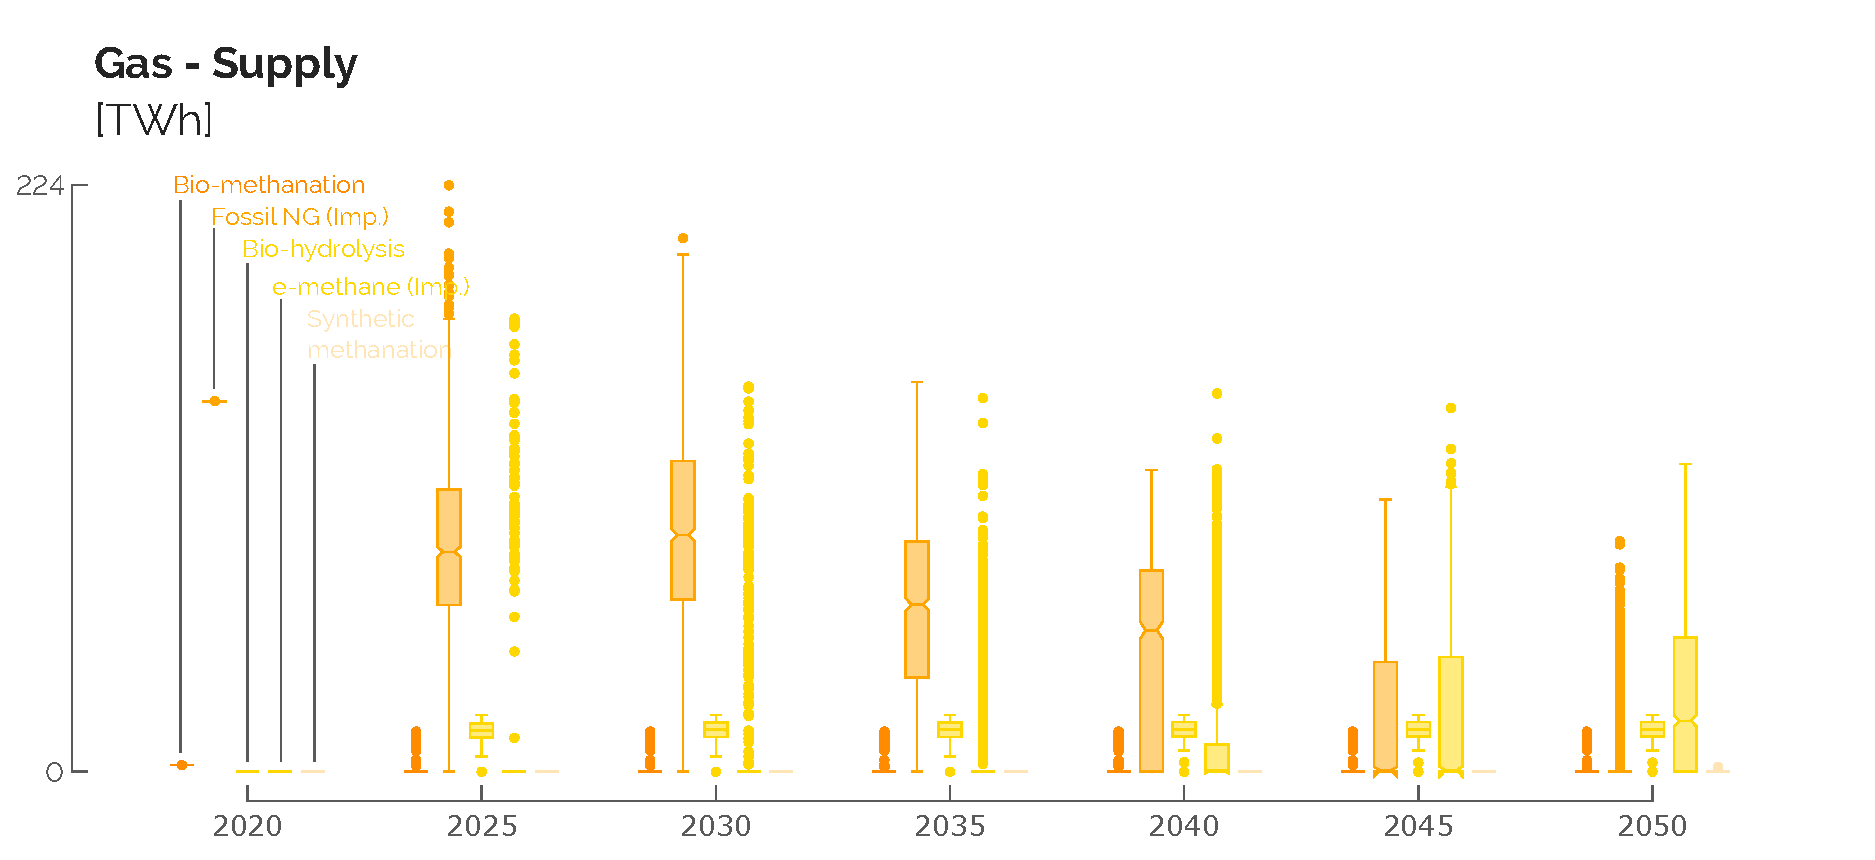
\includegraphics[width=0.49\textwidth]{UQ_Gas_Prod.pdf}
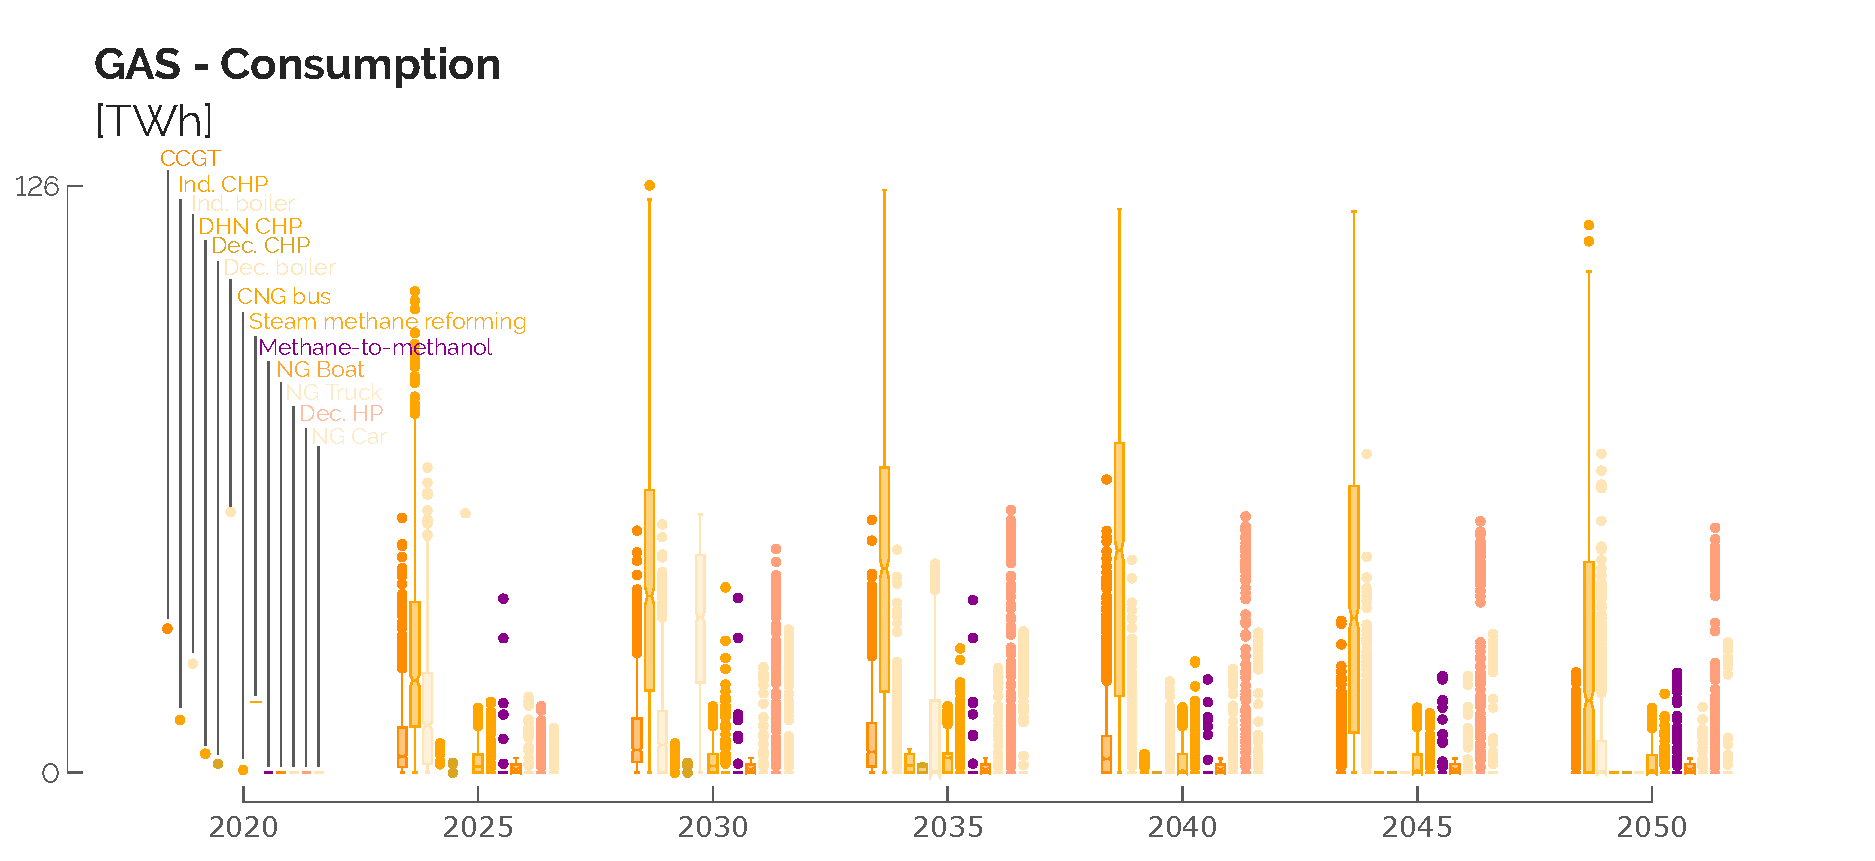
\includegraphics[width=0.49\textwidth]{UQ_Gas_Cons.pdf}
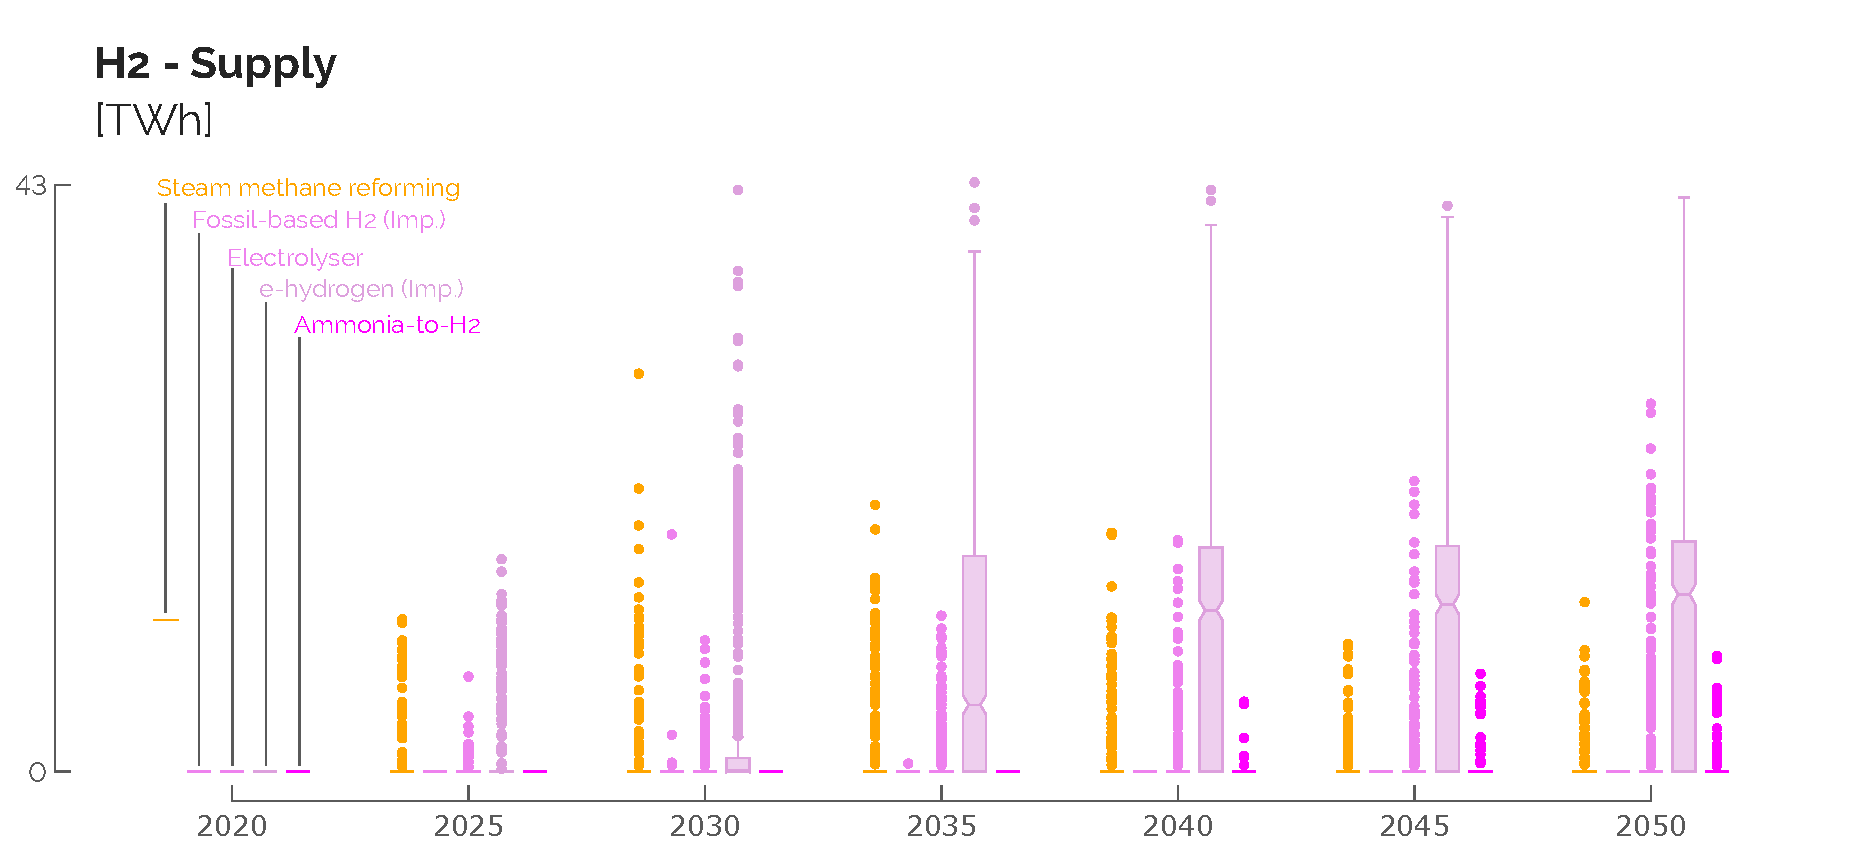
\includegraphics[width=0.49\textwidth]{UQ_H2_Prod.pdf}
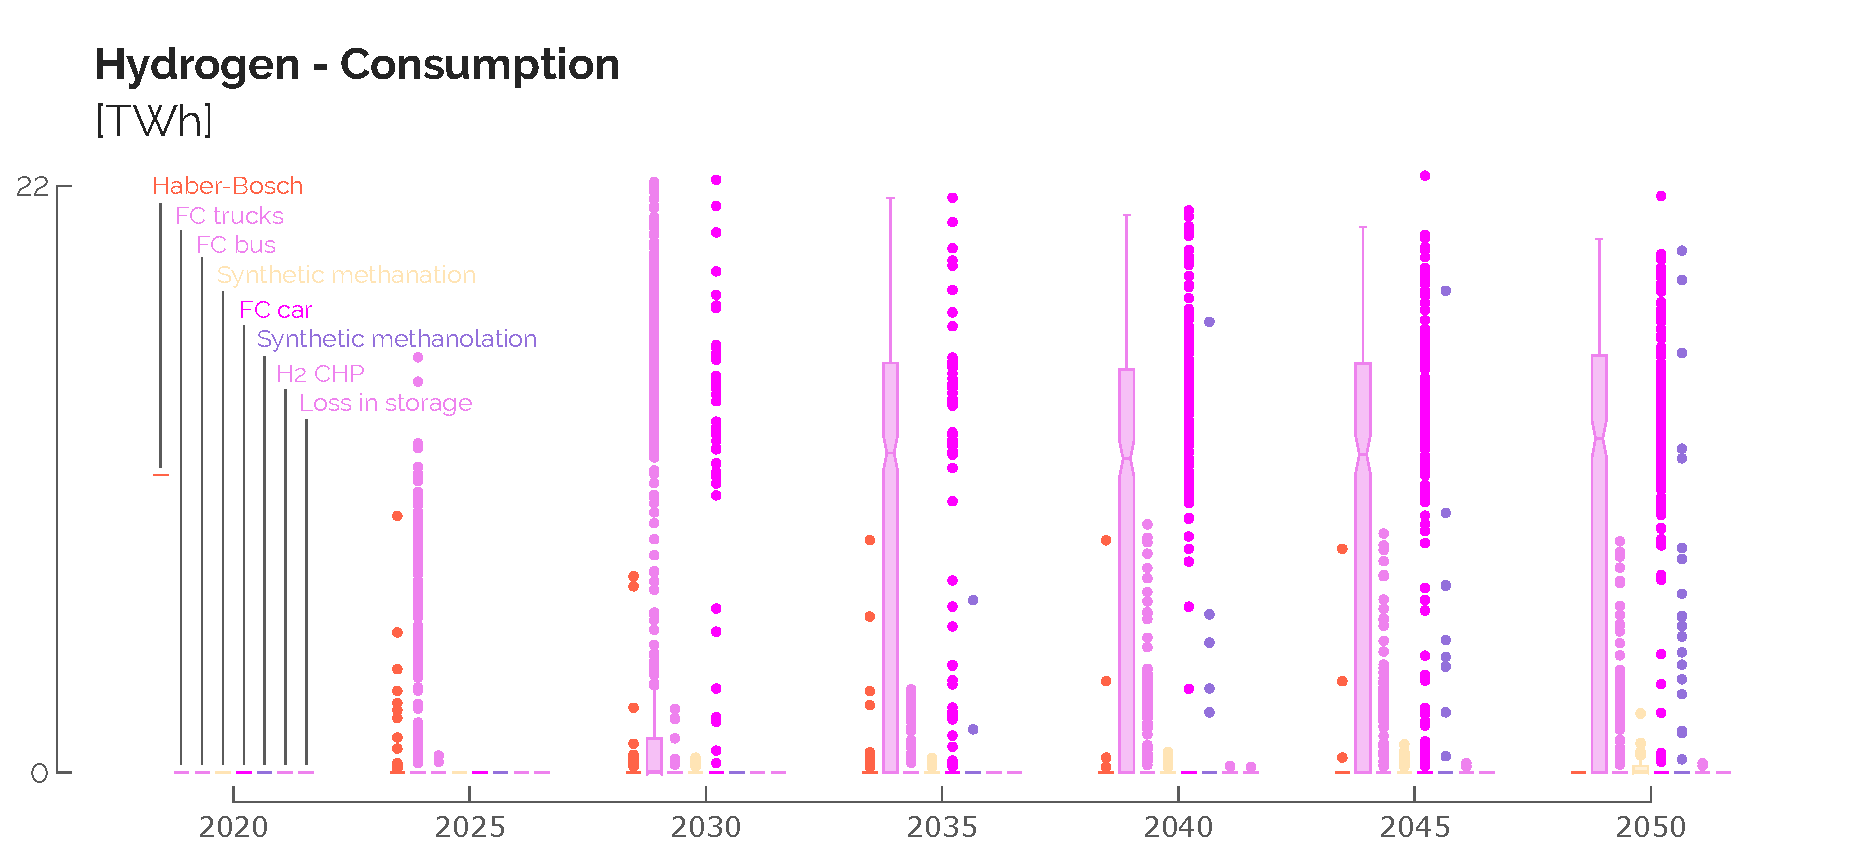
\includegraphics[width=0.49\textwidth]{UQ_H2_Cons.pdf}
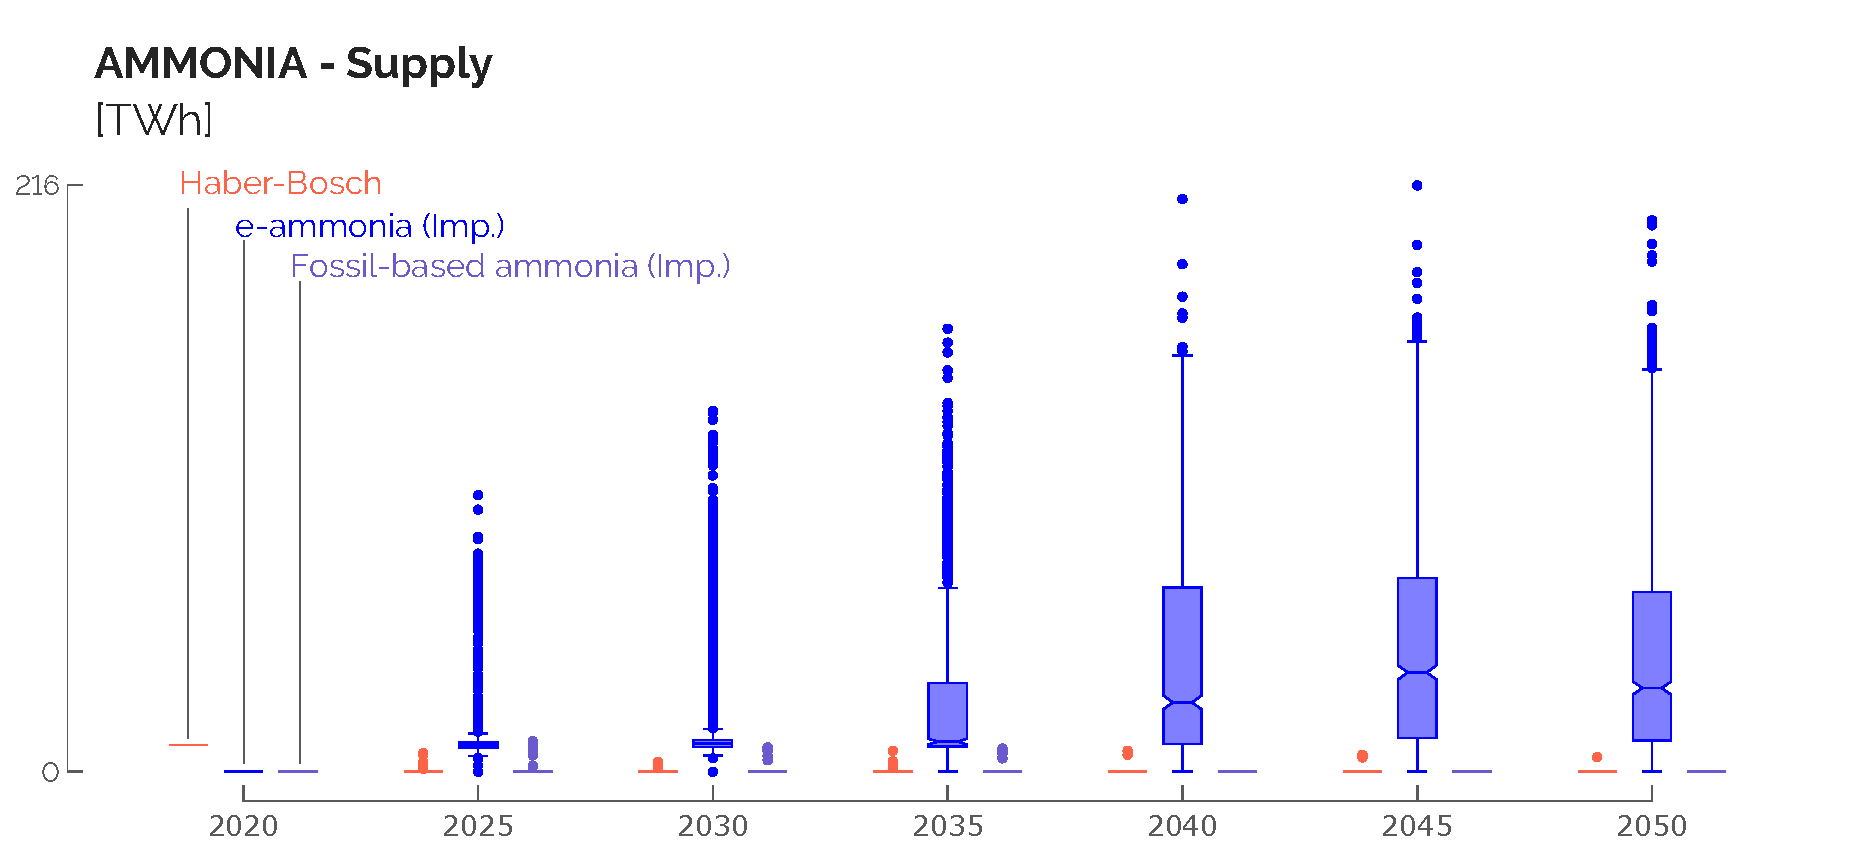
\includegraphics[width=0.49\textwidth]{UQ_Ammonia_Prod.pdf}
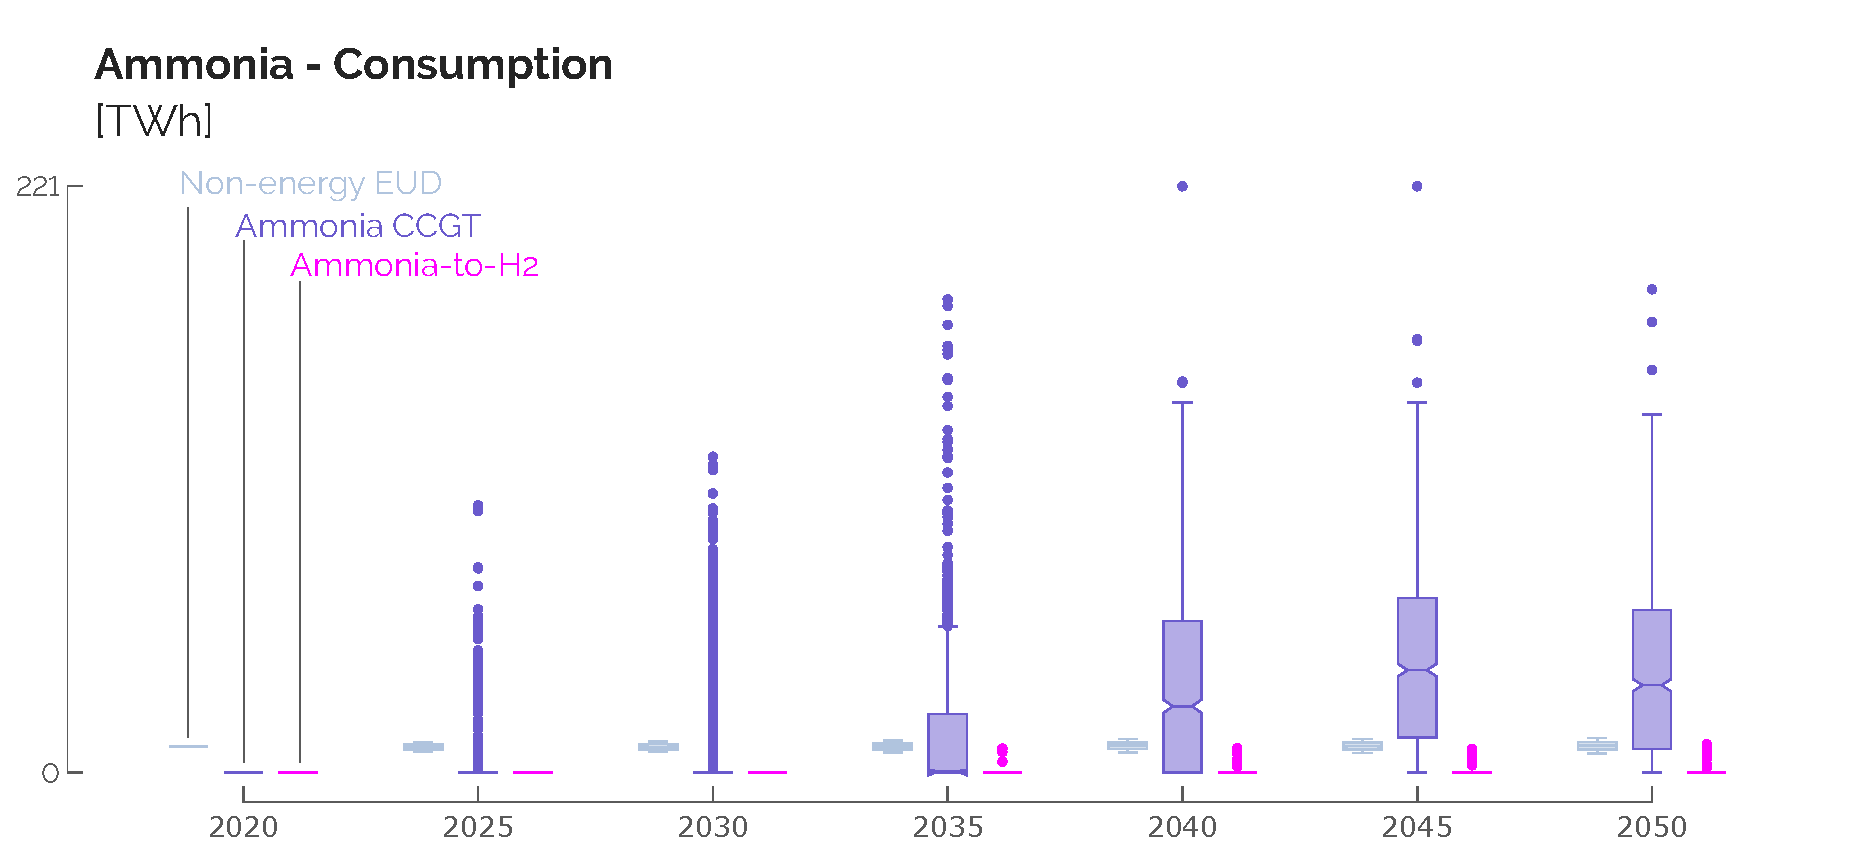
\includegraphics[width=0.49\textwidth]{UQ_Ammonia_Cons.pdf}
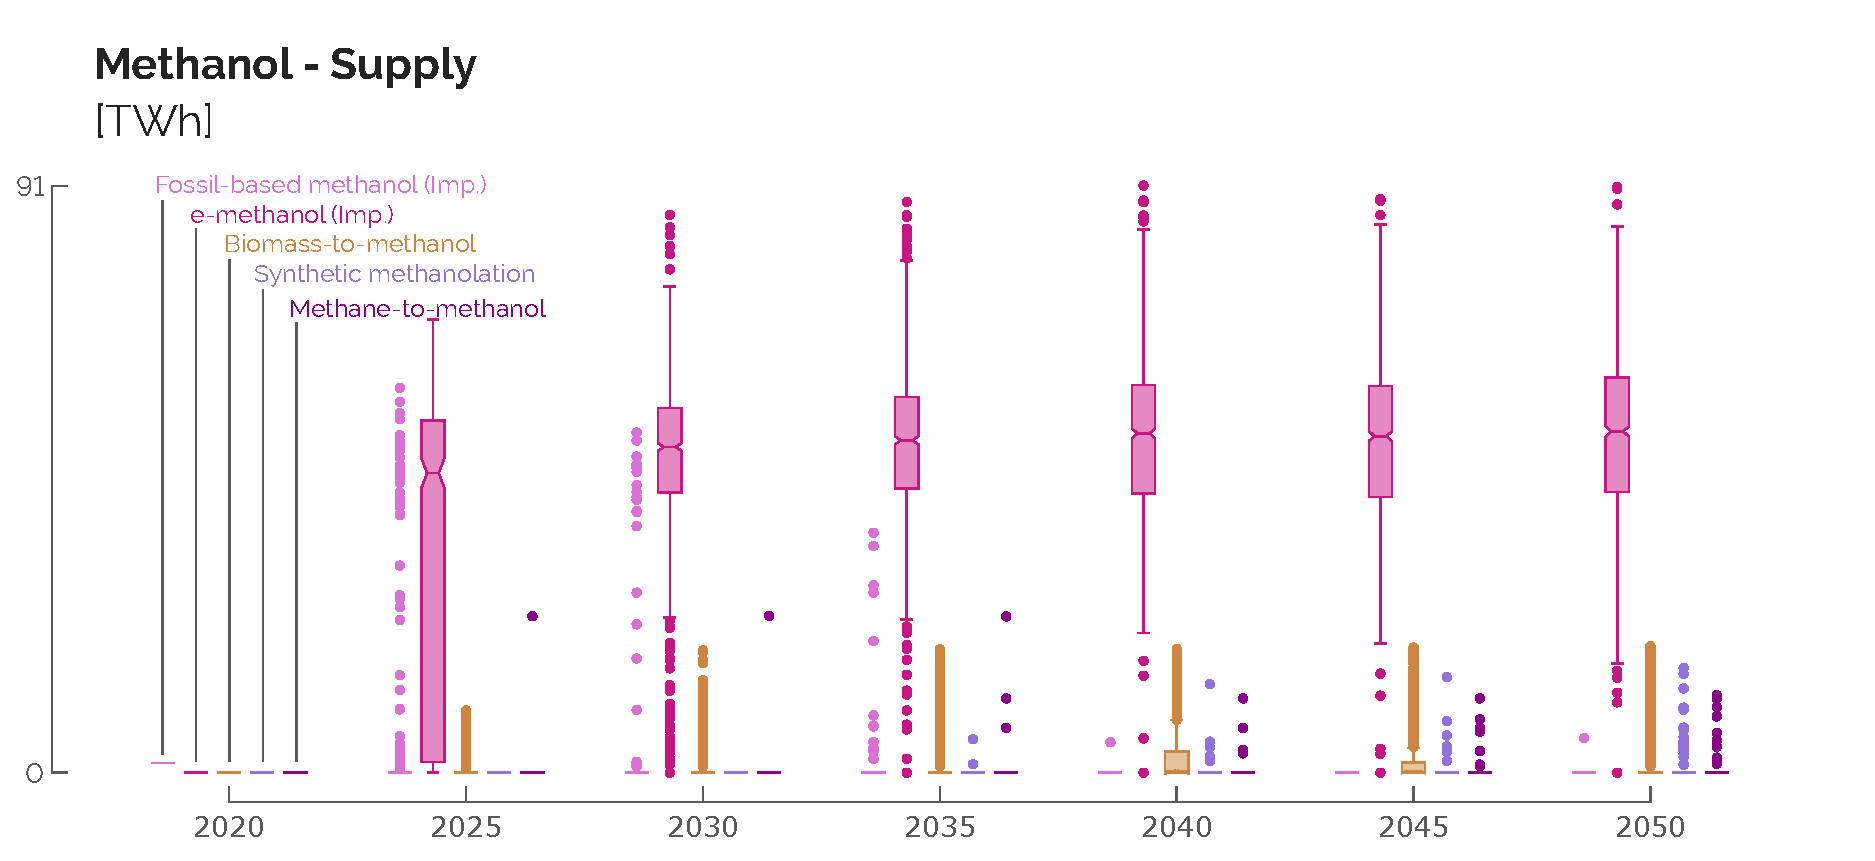
\includegraphics[width=0.49\textwidth]{UQ_Methanol_Prod.pdf}
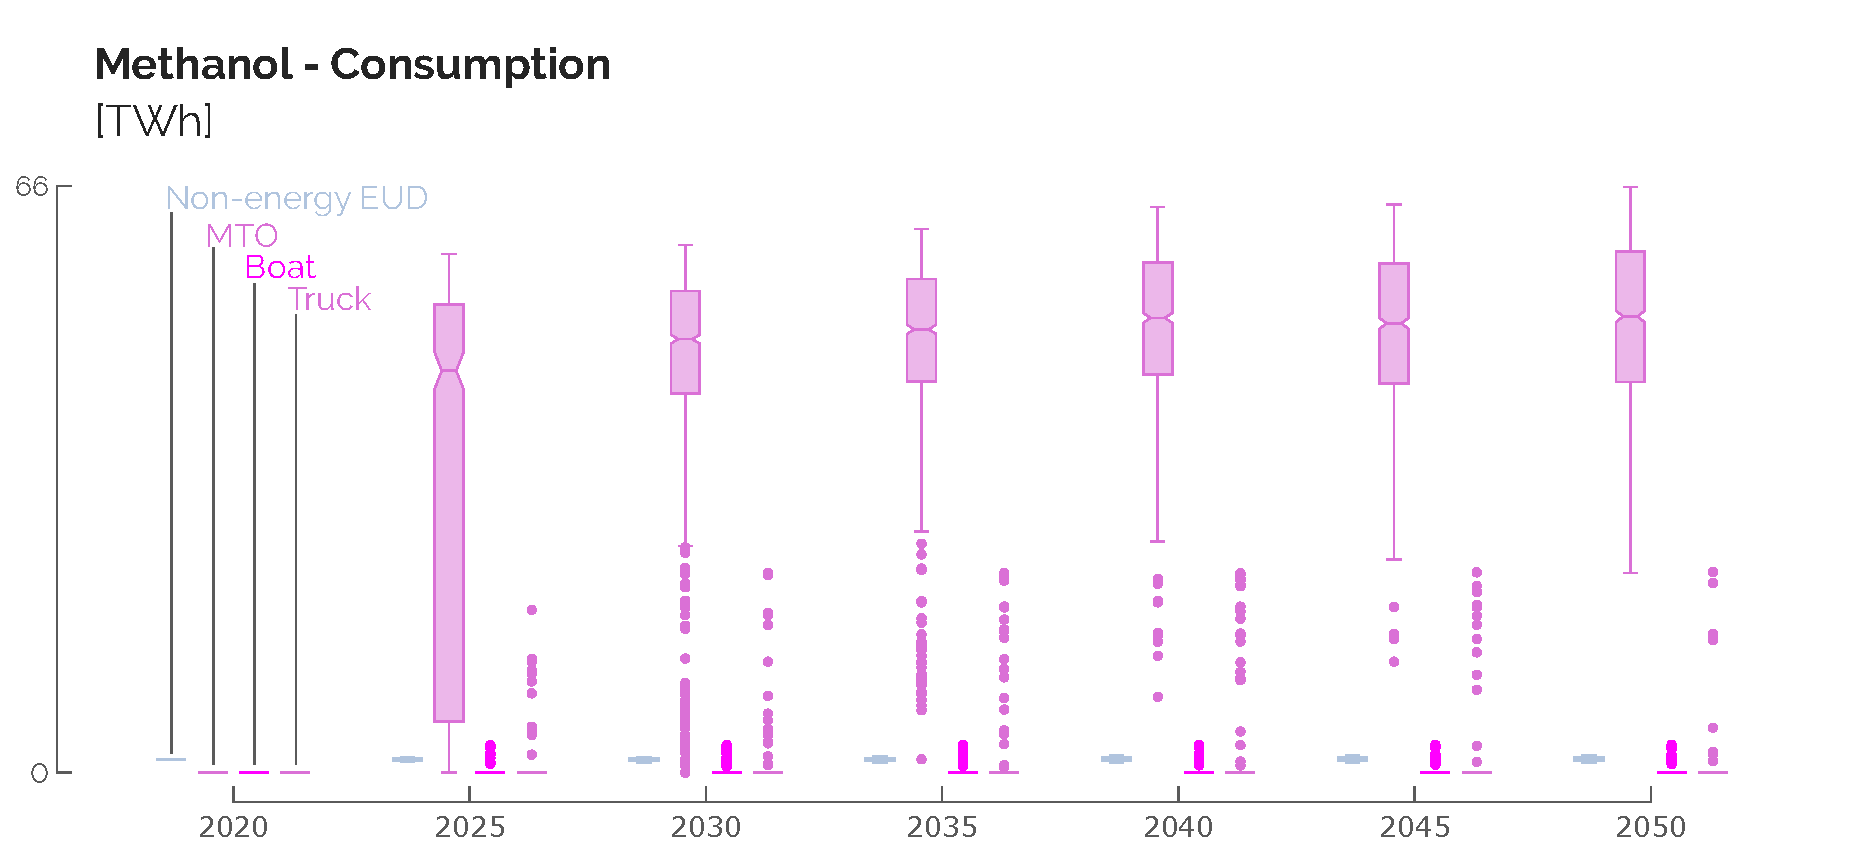
\includegraphics[width=0.49\textwidth]{UQ_Methanol_Cons.pdf}
\caption{Distribution of the different streams of supply (left) and consumption (right) of gas, hydrogen, ammonia and methanol from the \acrfull{GSA}.}
\label{fig:results_uq_prod_cons}
\end{figure}

\newpage
\section{Installed capacities}
\label{app:UQ_tech_cap}

\begin{figure}[htbp!]
\centering
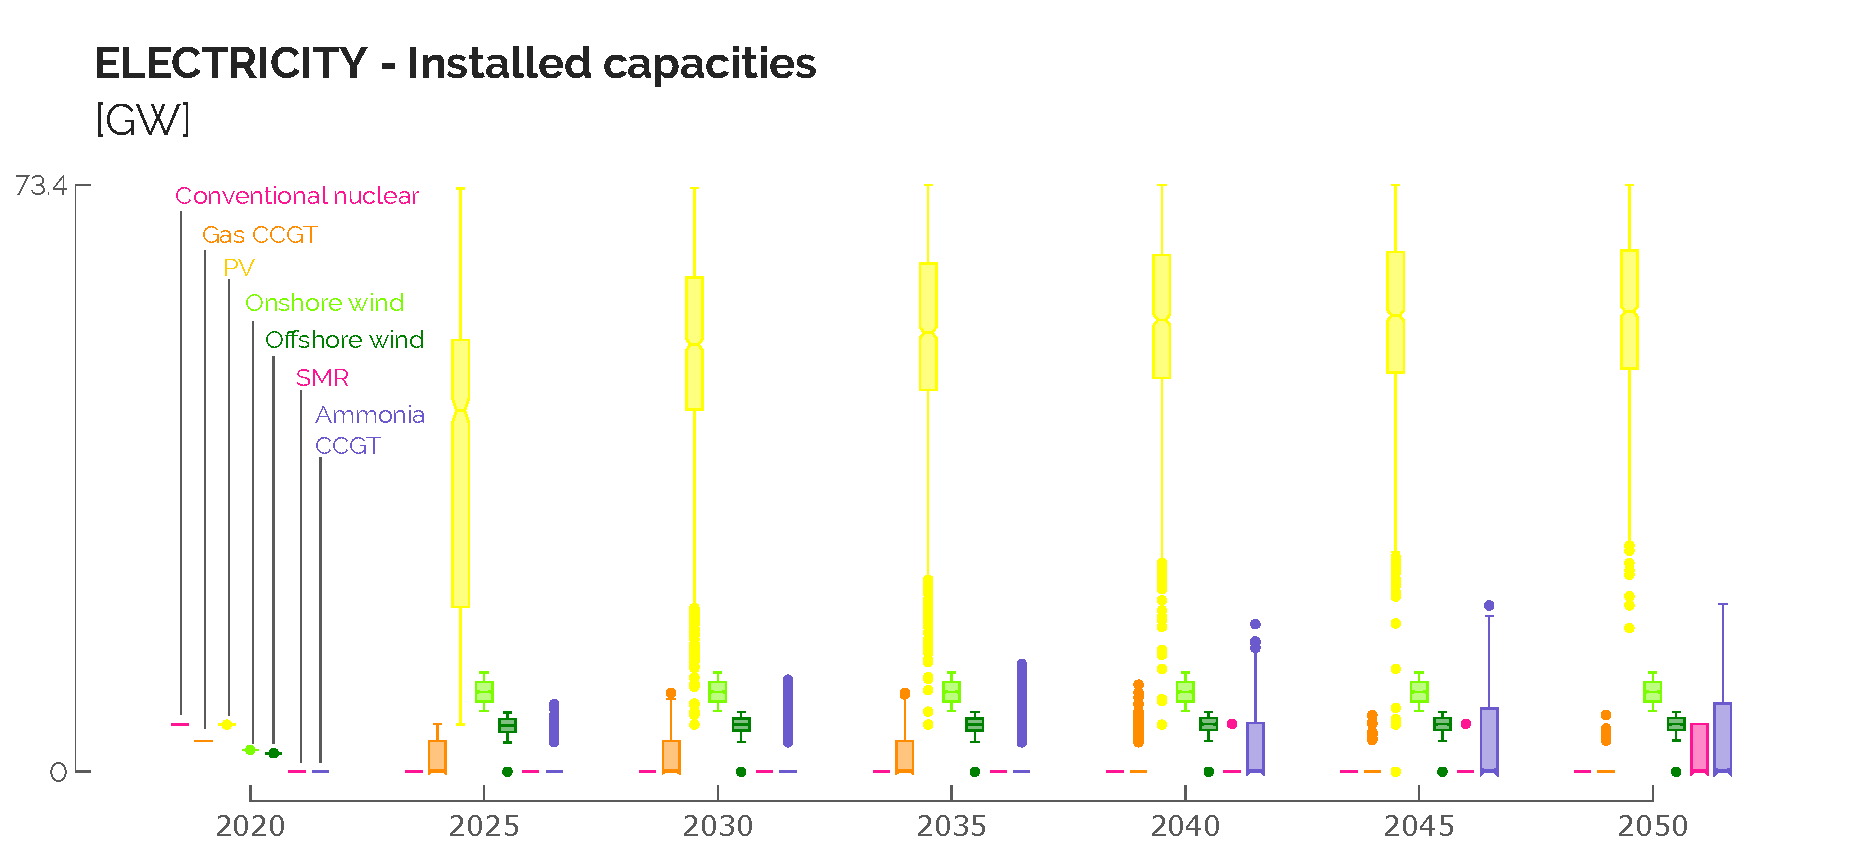
\includegraphics[width=0.49\textwidth]{ELECTRICITY_Tech.pdf}
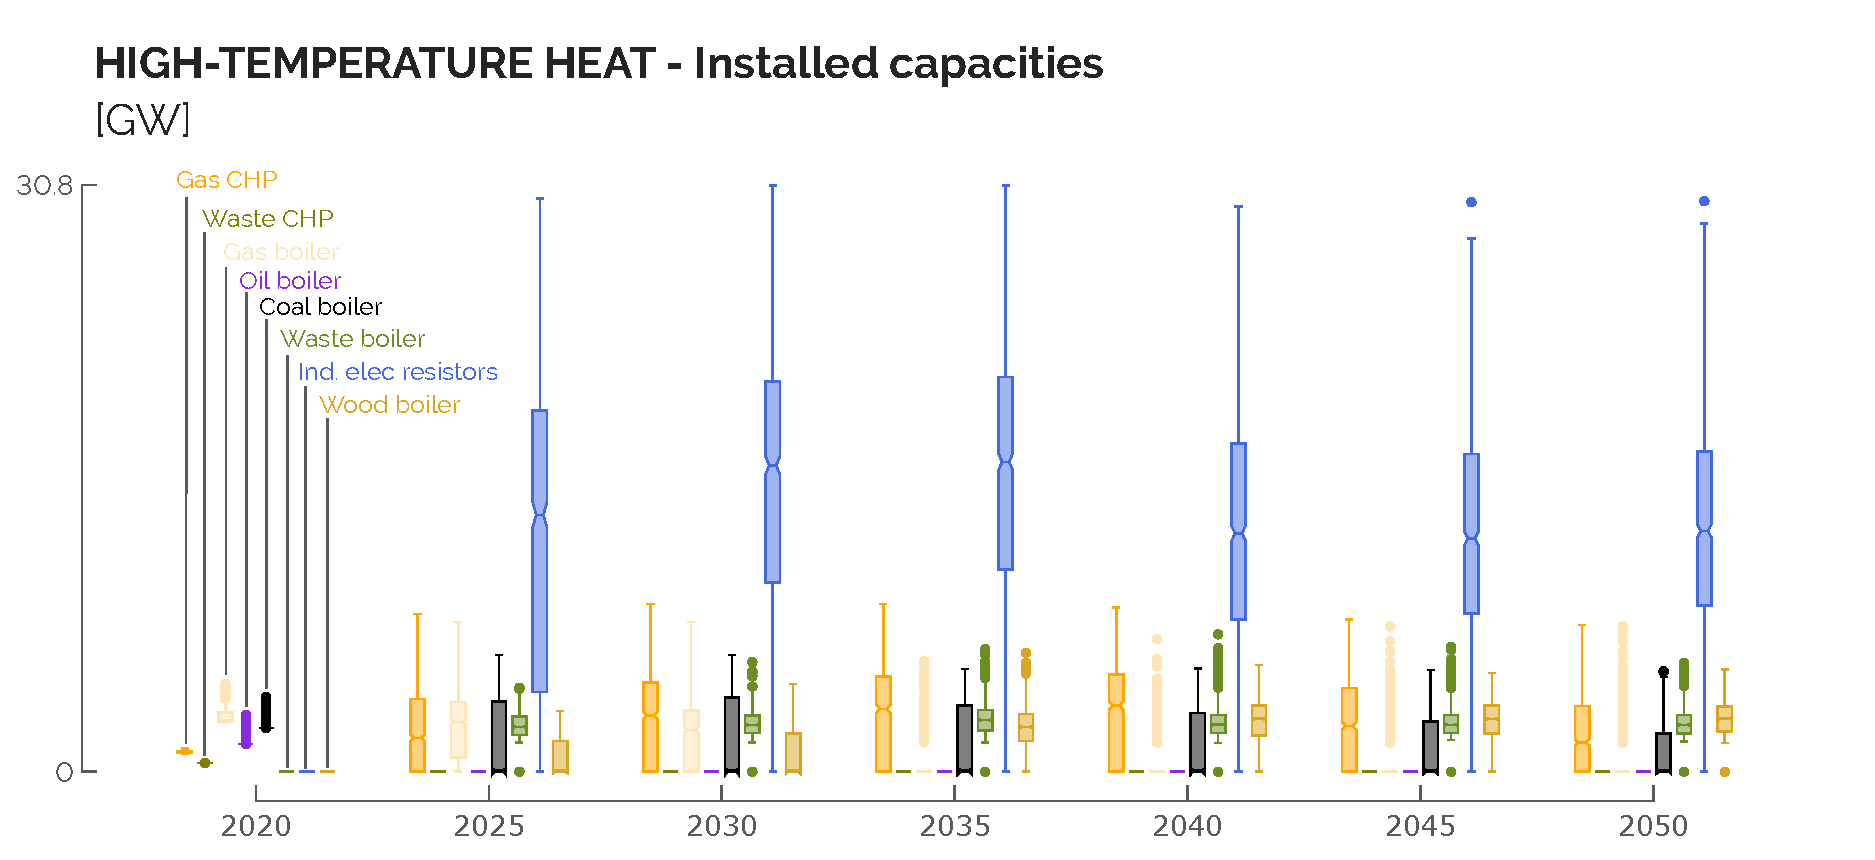
\includegraphics[width=0.49\textwidth]{HT_HEAT_Tech.pdf}
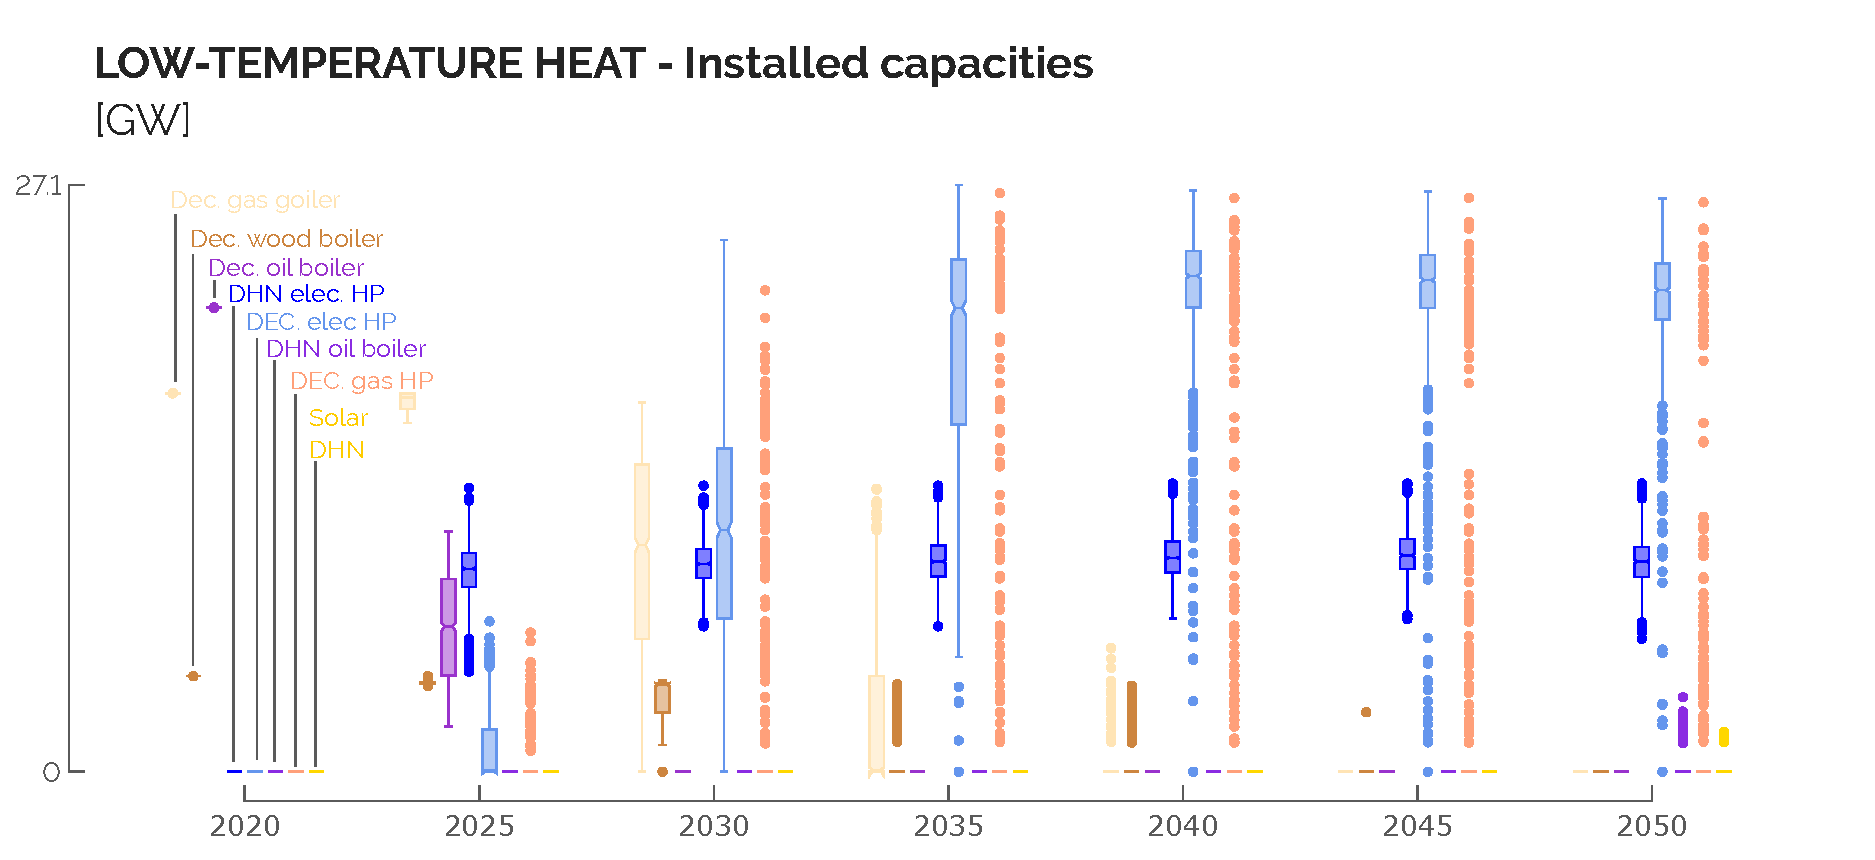
\includegraphics[width=0.49\textwidth]{LT_HEAT_Tech.pdf}
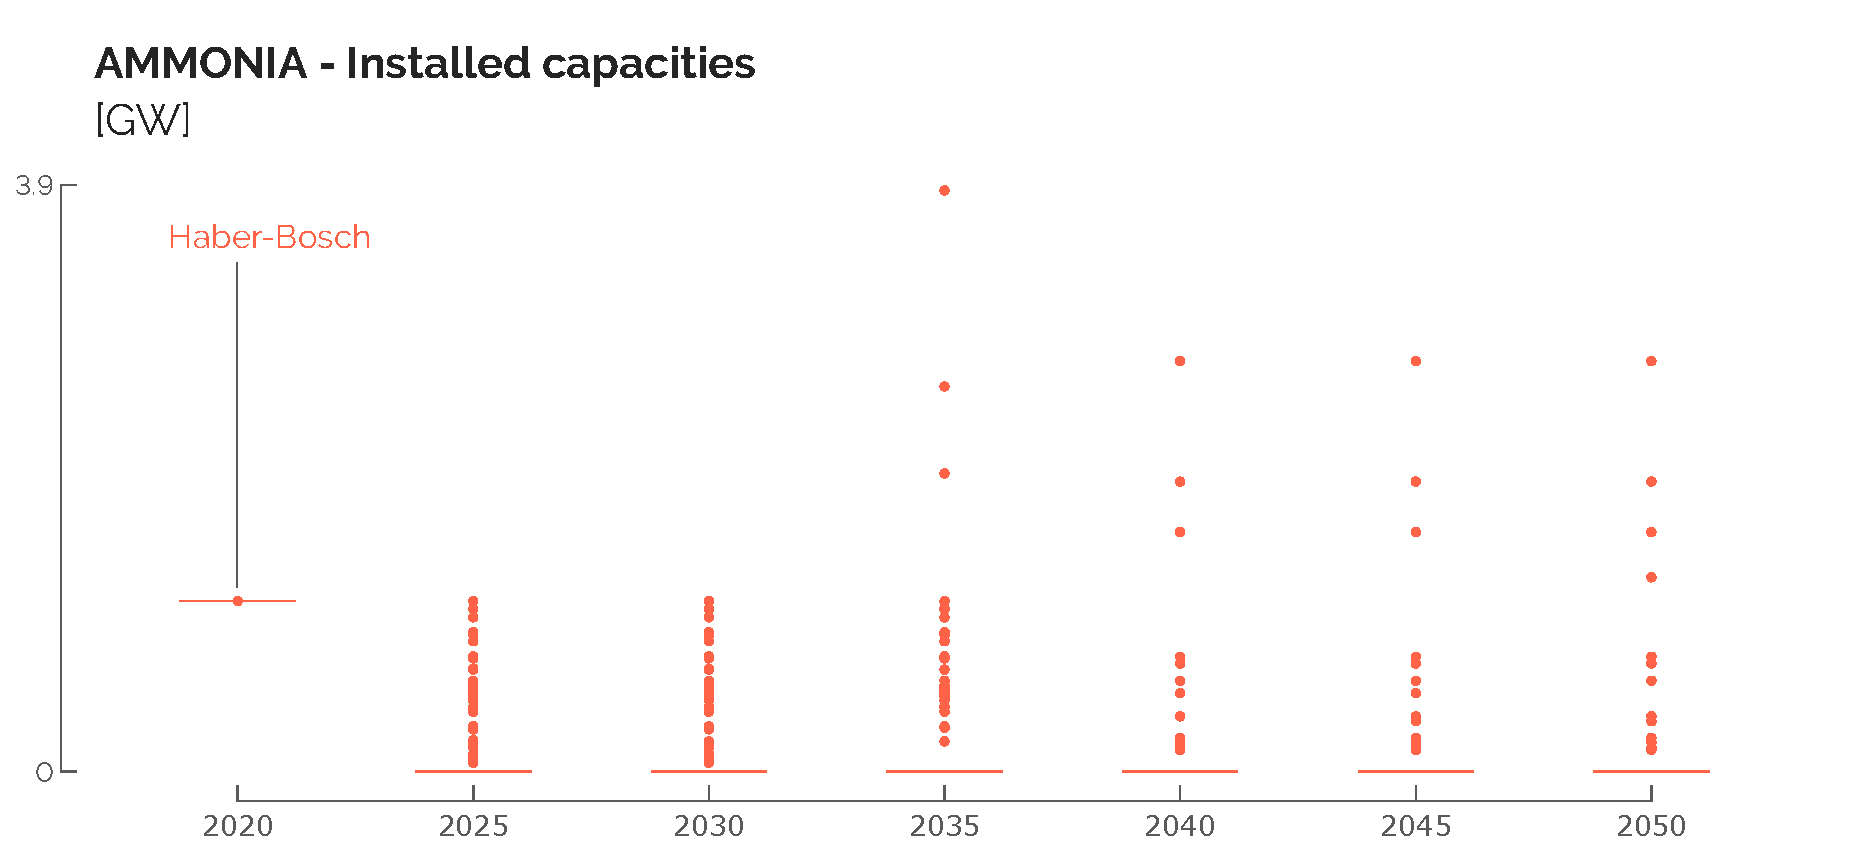
\includegraphics[width=0.49\textwidth]{AMMONIA_Tech.pdf}
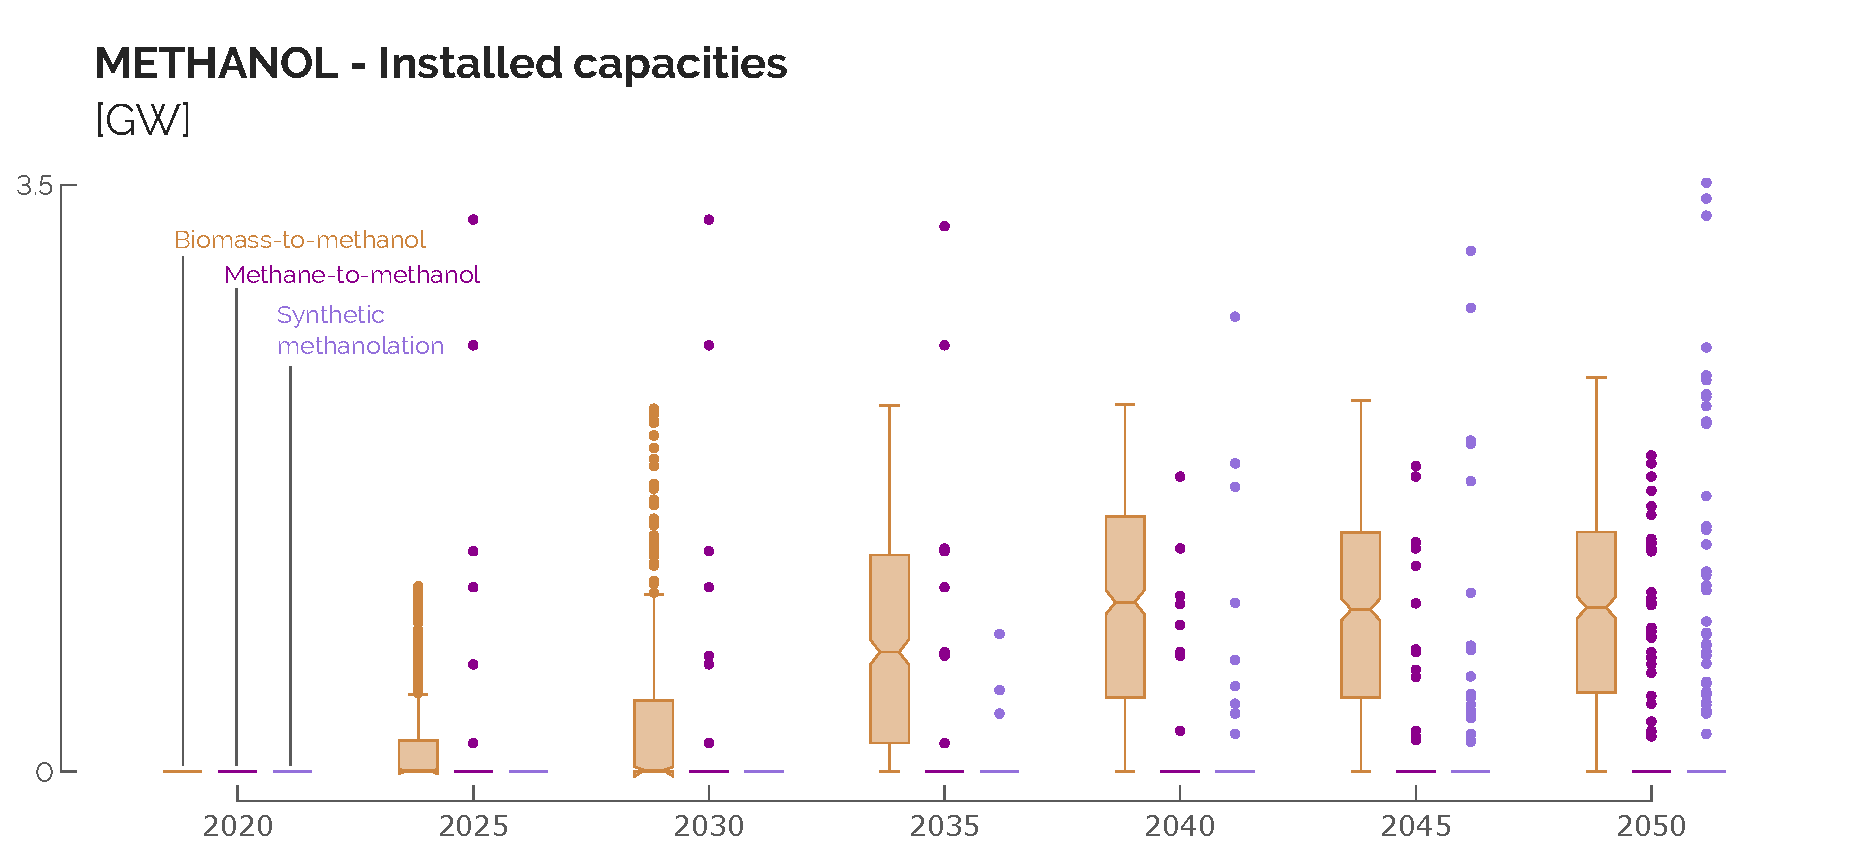
\includegraphics[width=0.49\textwidth]{METHANOL_Tech.pdf}
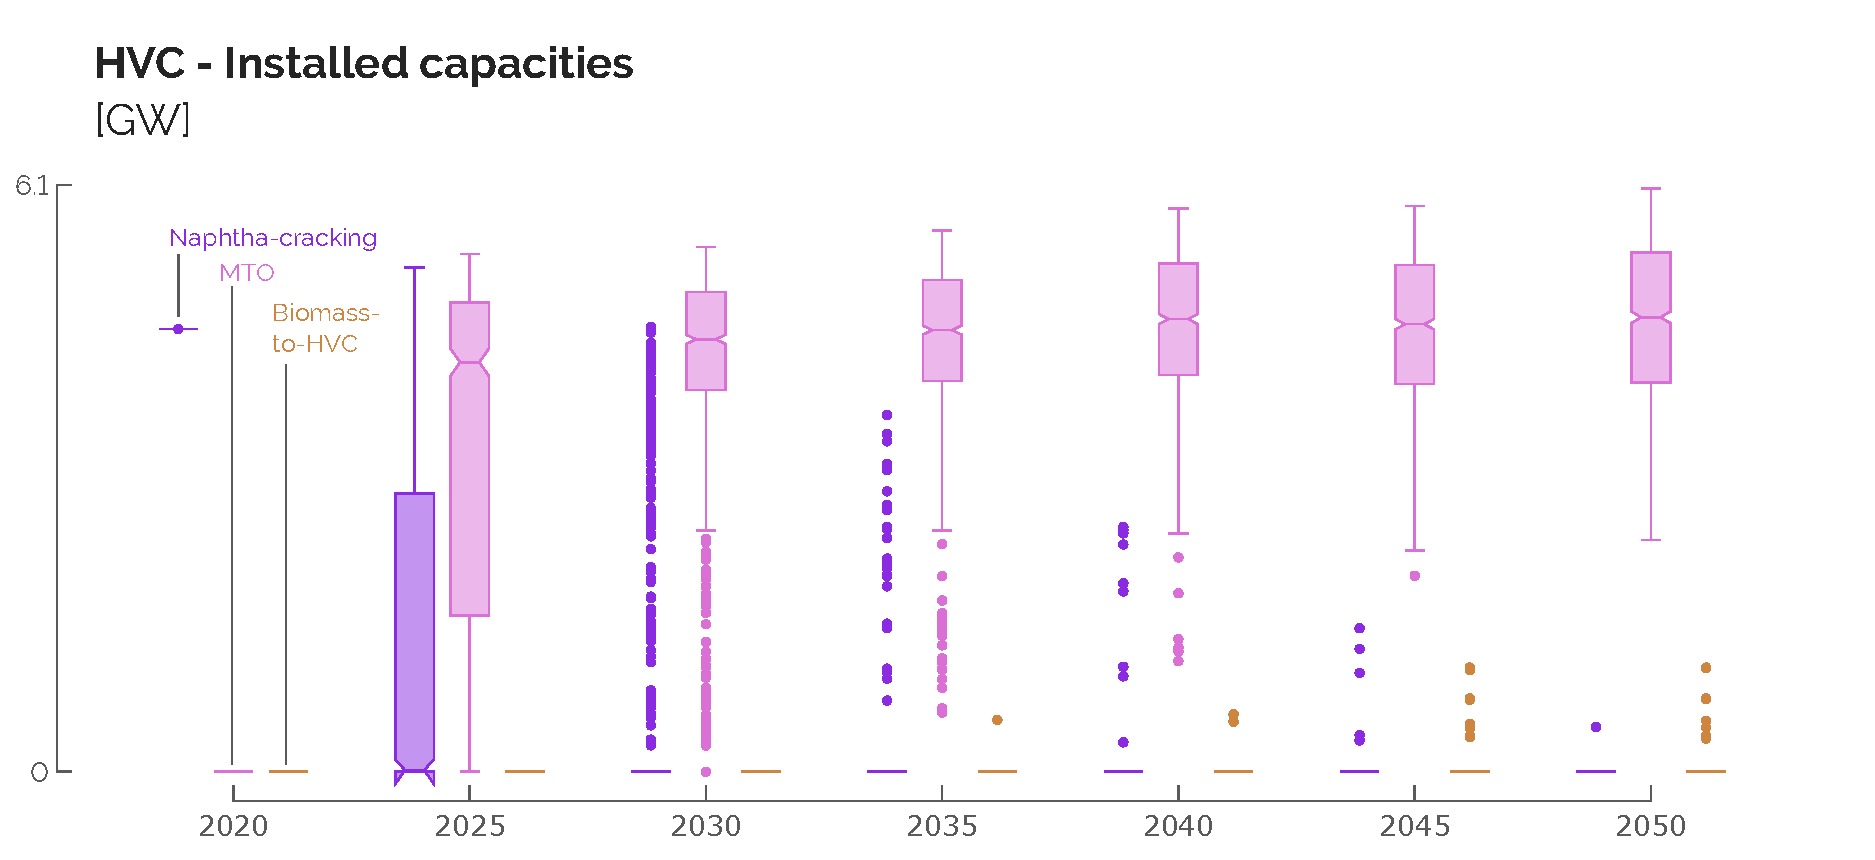
\includegraphics[width=0.49\textwidth]{HVC_Tech.pdf}
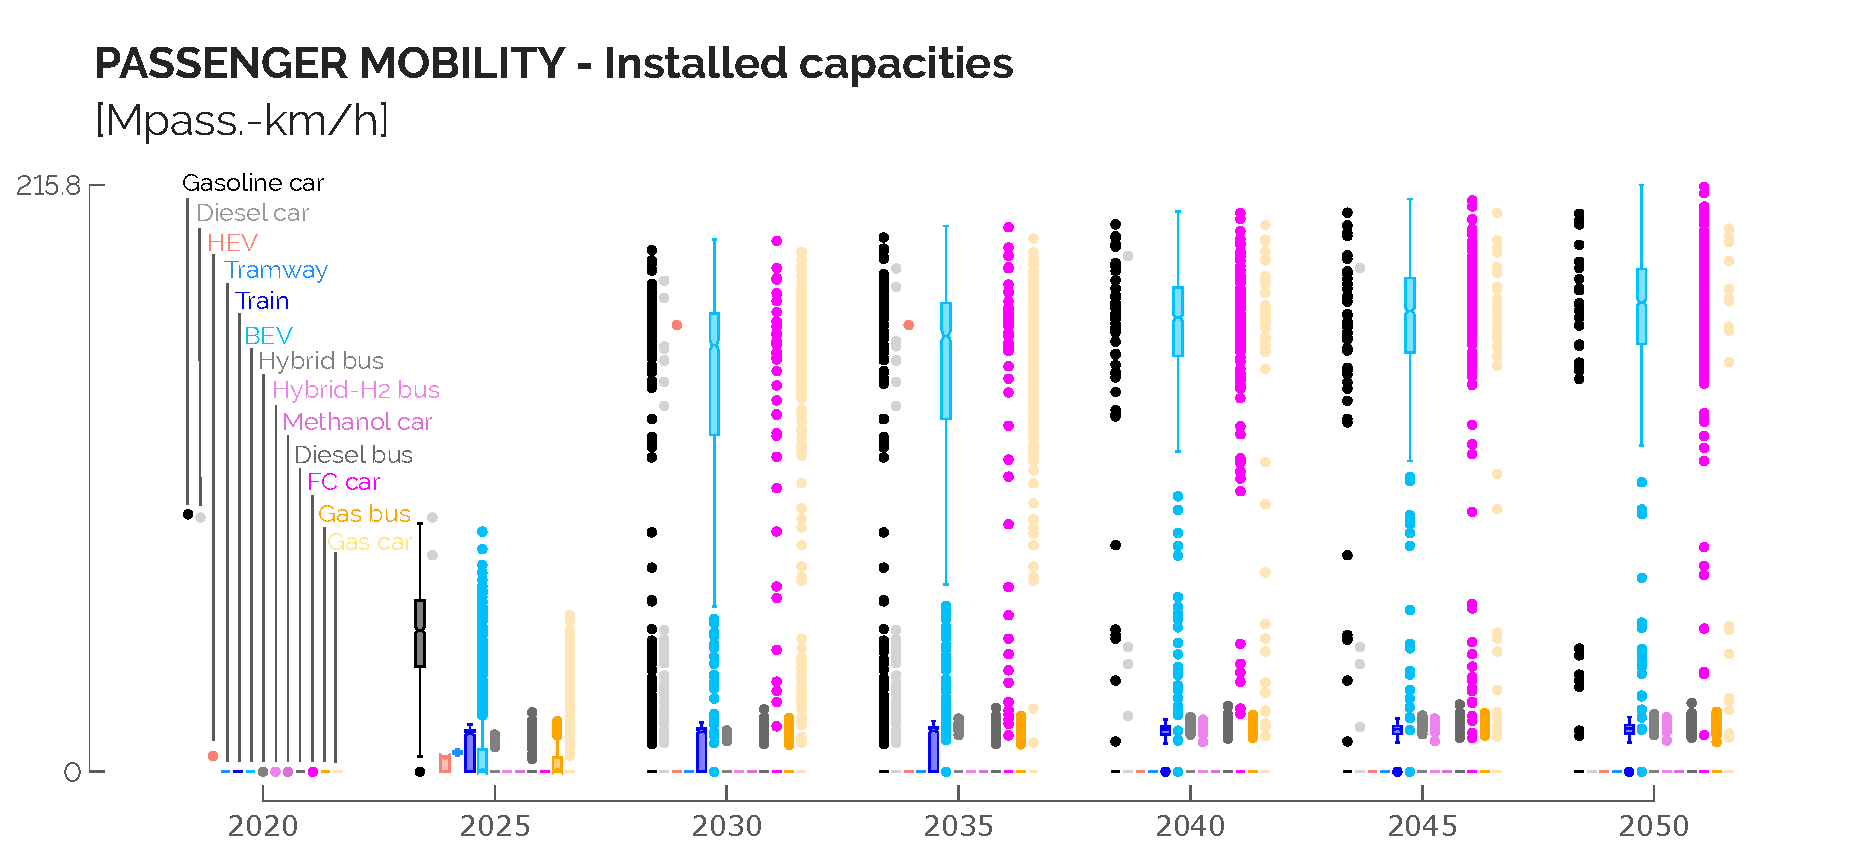
\includegraphics[width=0.49\textwidth]{PASS_MOB_Tech.pdf}
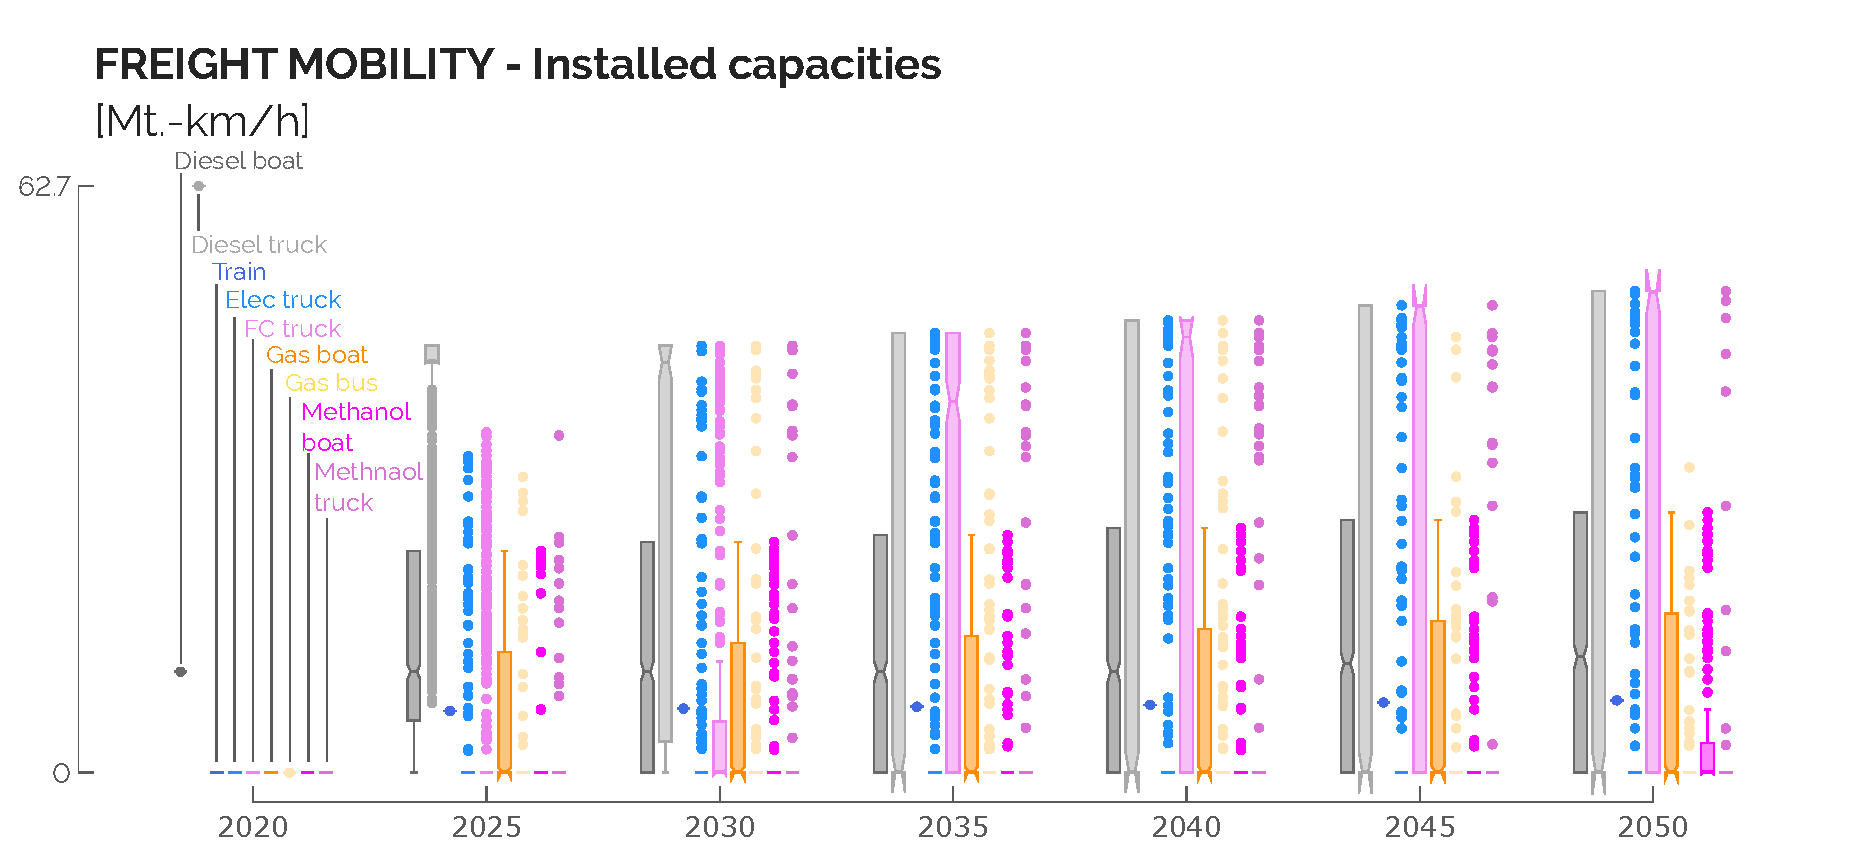
\includegraphics[width=0.49\textwidth]{FREIGHT_MOB_Tech.pdf}
\caption{Distribution of the installed capacities among the different end-use sectors from the \acrfull{GSA}.}
\label{fig:results_uq_tech_cap}
\end{figure}